Haskind-relasjonene finner vi fra følgende 
\begin{equation}
\frac{X_2}{\mathrm{i} \omega \rho}  =  - \int_{S_B}  ( \phi_0 n_2 + \phi_7 n_2) dS = - \int_{S_B}  \Big( \phi_0 \frac{\partial \phi_2}{\partial n} + \phi_7 \frac{\partial \phi_2}{\partial n} \Big),
\end{equation}
der randverdibetingelsen $\frac{\partial \phi_2}{\partial n} = n_2$ er brukt. Videre har vi at potensialet $\phi_2$ og $\phi_7$ tilfredstiller den samme randa ved: 
\begin{description}
\item[a)] Den frie overflaten, der $-\omega^2 \phi_{2,7} + g\frac{\partial \phi_{2,7}}{\partial y} = 0$, ved $y=0$ 
\item[b)] $\frac{\partial \phi_{2,7}}{\partial n} = -\mathrm{i} K \phi_{2,7}$, i fjernfeltet ved $x = \pm \infty$
\item[c)]  $|\nabla \phi_{2,7} \rightarrow 0 |$, på dypet $y  \rightarrow -\infty$
\end{description}

dette gir at 
\begin{equation}
\int_{S_B}  \big( \phi_7 \frac{\partial \phi_2}{\partial n} -\phi_0 \frac{\partial \phi_2}{\partial n}  \big) = 0. 
\end{equation}

%hopper
%% ned til 
%

Første haskind-relasjon
\begin{equation}
\frac{X_2^{\text{Haskind v1}}}{i \omega \rho} = -\int_{S_B}  \big( \phi_0 \frac{\partial \phi_2}{\partial n} -\phi_2 \frac{\partial \phi_0}{\partial n}  \big) dS 
\end{equation}

Andre haskind-relasjon
\begin{equation}
\frac{X_2^{\text{Haskind v2}}}{i \omega \rho} = \int_{S_\infty}  \big( \phi_0 \frac{\partial \phi_2}{\partial n} -\phi_2 \frac{\partial \phi_0}{\partial n}  \big) dS, 
\end{equation}
Fjernfeltet $\phi_2$ er gitt ved
\begin{align}
\phi_2 = A_2^{\pm \infty}e^{K (\bar{y} \pm \mathrm{i}  \bar{x}) },  \quad x \rightarrow\pm \infty
\end{align}
der
\begin{align}
A_2^{\pm \infty} =  \mathrm{i} \int_{S_B}   \bigg[ \phi_2  \Big(  n_1 \frac{\partial }{\partial x}  +  n_2\frac{\partial }{\partial y} \Big) - n_2 \bigg]  e^{K (\bar{y} \pm \mathrm{i}  \bar{x})} dS
\end{align}
%%%

setter inn i likningen for Haskind2
$\phi_0 = \frac{\mathrm{i} g}{\omega} e^{K (\bar{y} \pm \mathrm{i}  \bar{x})}$, og $\frac{\partial \phi_2}{\partial n} = -n_2$, og $\frac{\partial \phi_0}{\partial n} = \frac{\mathrm{i} g}{\omega} e^{K (\bar{y} \pm \mathrm{i}  \bar{x})} * (kjernen derivert?)$.

\textcolor{red}{
\begin{equation}
\frac{X_2^{\text{H2}}}{\mathrm{i} \omega \rho} = \int_{S_\infty}  \big( -\frac{\mathrm{i} g}{\omega} e^{K (\bar{y} \pm \mathrm{i}  \bar{x})} n_2 -\phi_2\frac{\mathrm{i} g}{\omega} e^{K (\bar{y} \pm \mathrm{i}  \bar{x})} * (??)  \big) dS, 
\end{equation}
\begin{equation}
\frac{X_2^{\text{H2}}}{\rho g\cancel{\omega}  } = \frac{\mathrm{i} \cdot \mathrm{i} }{\cancel{\omega}}  \int_{S_\infty}  \big[ -n_2 -\phi_2 * (??)  \big]  e^{K (\bar{y} \pm \mathrm{i}  \bar{x})} dS, 
\end{equation}}

\begin{equation}
\frac{X_2^{\text{H2}}}{  \rho g} = \mathrm{i} \cdot \underbrace{\mathrm{i} \int_{S_\infty}  \big[ \phi_2(n_1\frac{\partial}{\partial x} + n_2\frac{\partial}{\partial y})   -n_2 \big]  e^{K (\bar{y} \pm \mathrm{i}  \bar{x})} dS}_{= A_2^{-\infty}}, 
\end{equation}

%% må vise stegene... 
\begin{equation}
\frac{X_2^{\text{Haskind v2}}}{i \omega \rho} = \mathrm{i}  A_2^{- \infty}, 
\end{equation}


%%%%- viser resultater under
\subsection{Nå sammenlikner vi eksitasjonskraften ved direkte integrering, Haskind 1 og 2, og Froude-Krylov-tilnærmingen.}

\noindent
\begin{minipage}[t]{0.45\linewidth}
    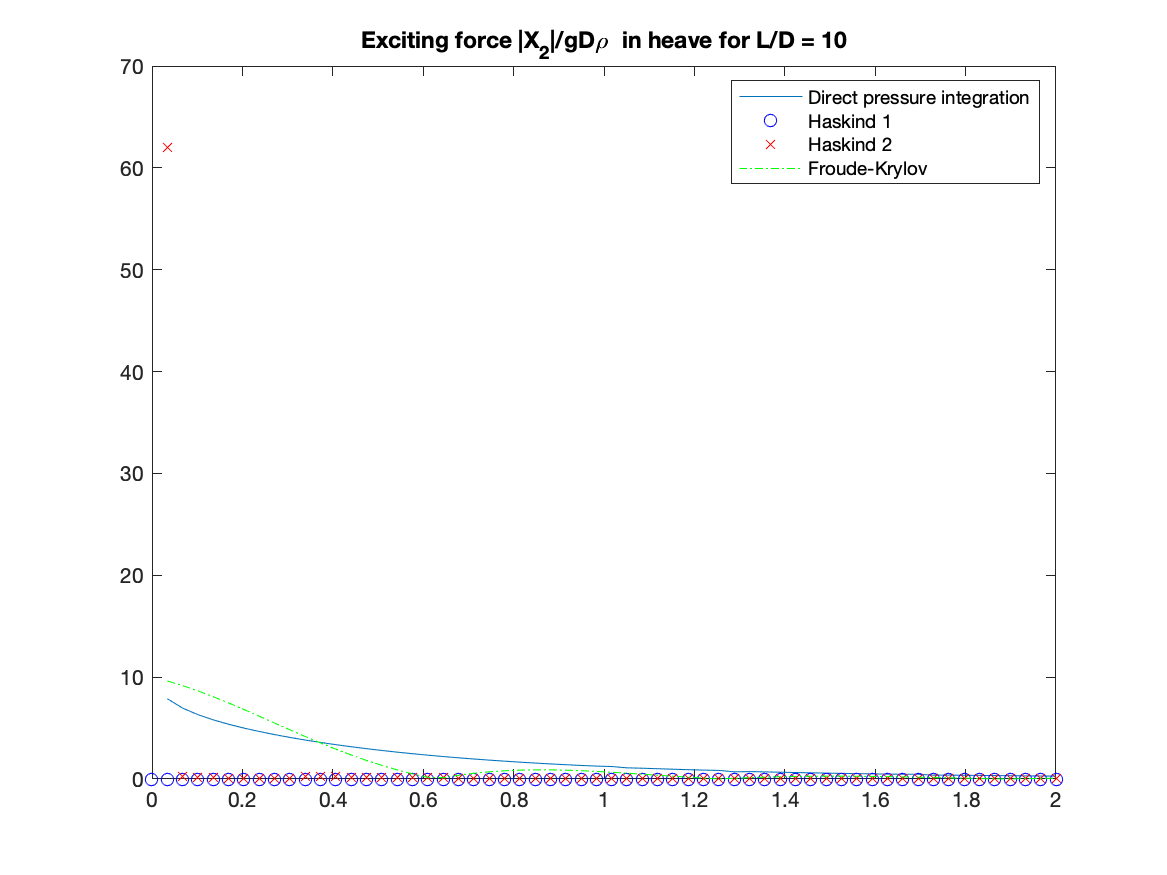
\includegraphics[width=\linewidth]{/Users/ole/Tex/MEK4420/oblig2images/aggregated_diffractionplot_1_LD_1.png}
    \captionof{figure}{L/D = 10}\label{fig:a22_1}
\end{minipage}
\hspace{0.05\linewidth}
\begin{minipage}[t]{0.45\linewidth}
    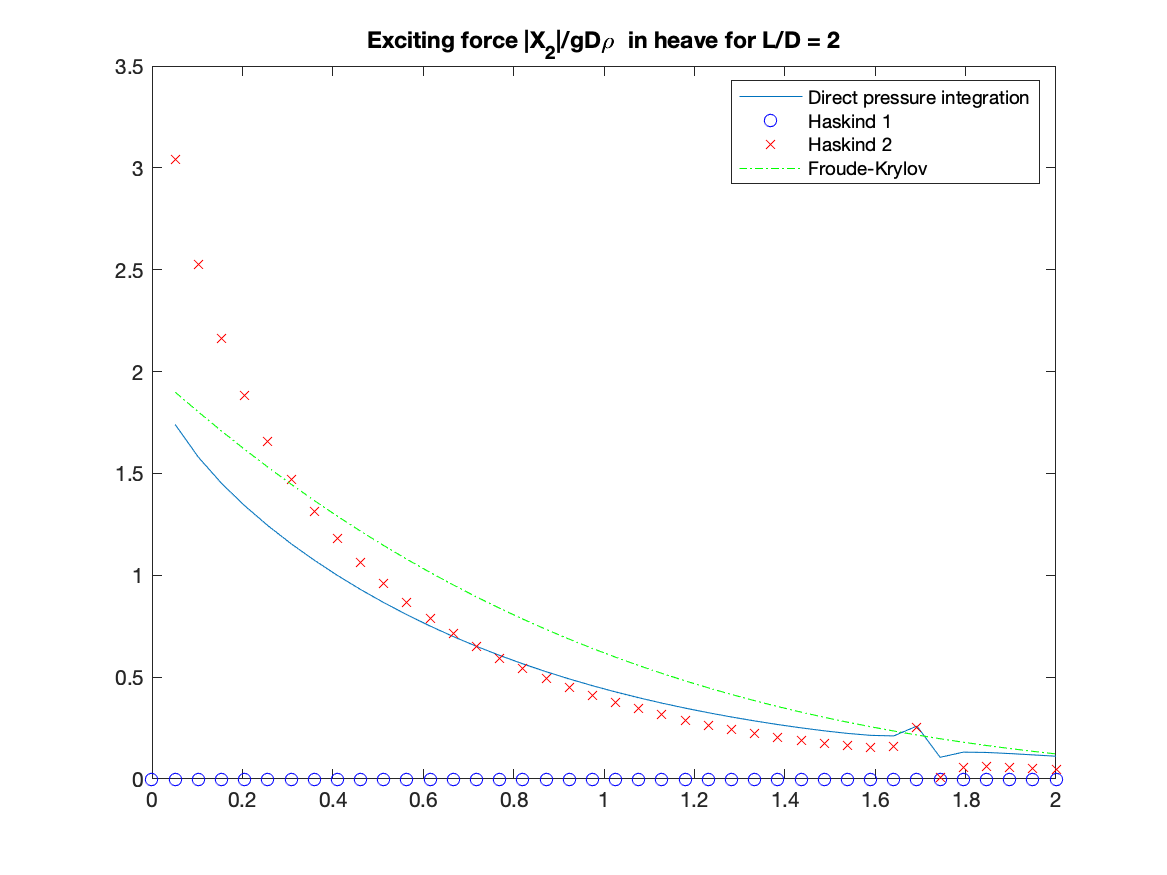
\includegraphics[width=\linewidth]{/Users/ole/Tex/MEK4420/oblig2images/aggregated_diffractionplot_2_LD_2.png}
    \captionof{figure}{L/D = 2}\label{fig:a22_2}
\end{minipage}

\vspace{0.5cm} % Adds vertical space between rows

\noindent
\begin{minipage}[t]{0.45\linewidth}
    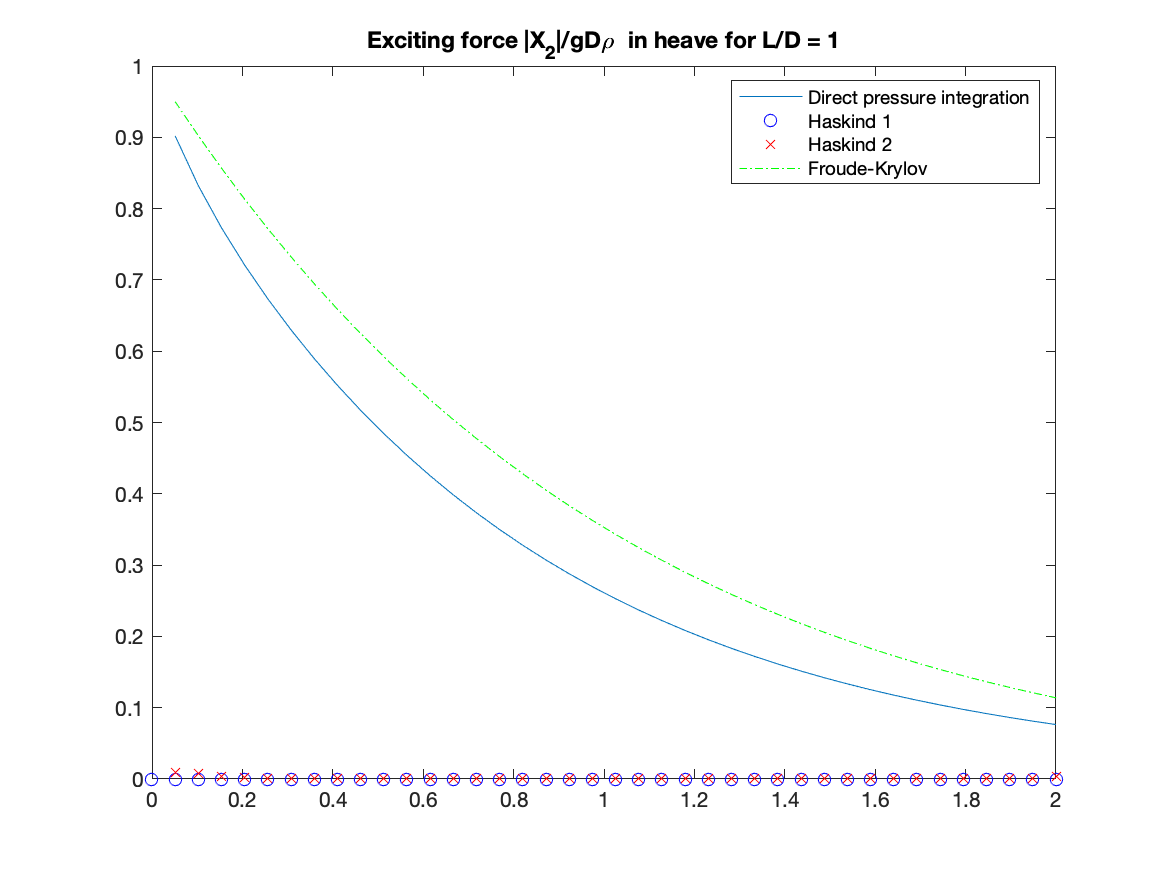
\includegraphics[width=\linewidth]{/Users/ole/Tex/MEK4420/oblig2images/aggregated_diffractionplot_3_LD_3.png}
    \captionof{figure}{L/D = 1}\label{fig:a22_3}
\end{minipage}
\hspace{0.05\linewidth}
\begin{minipage}[t]{0.45\linewidth}
    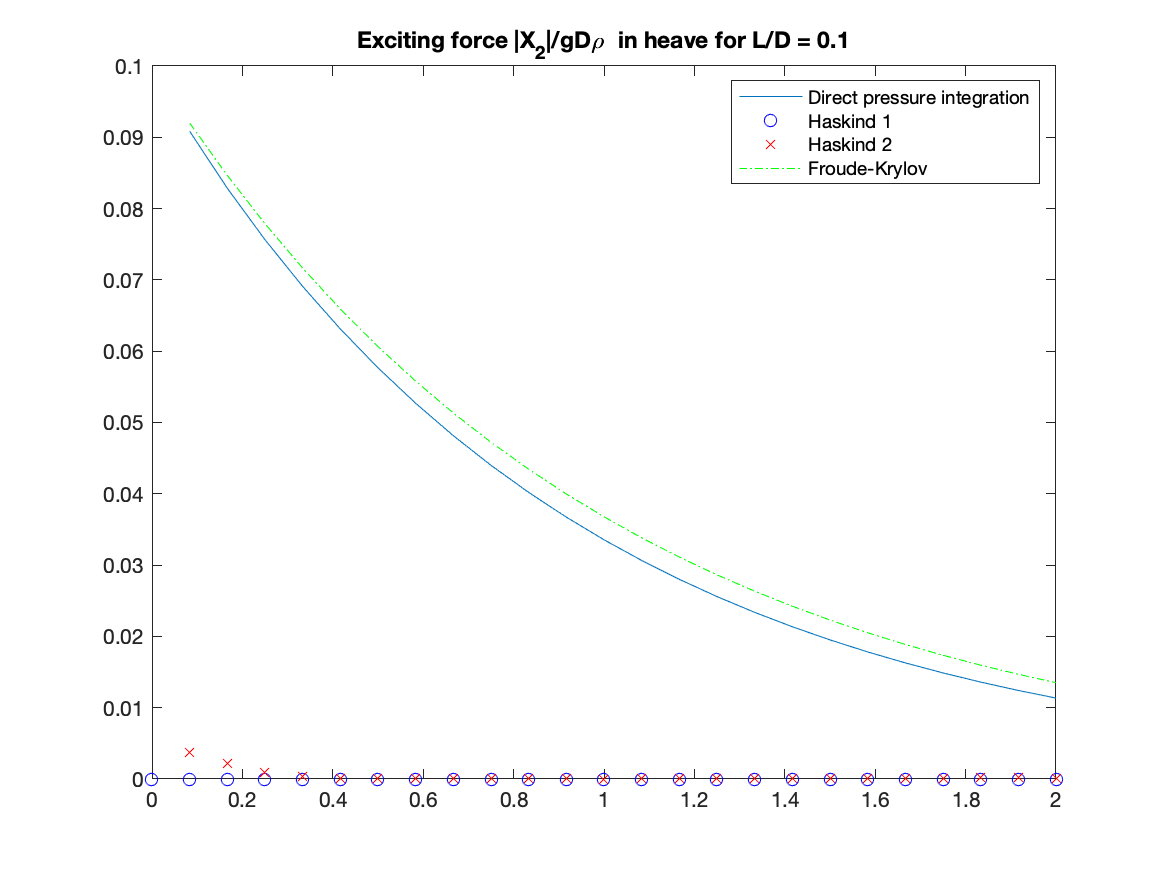
\includegraphics[width=\linewidth]{/Users/ole/Tex/MEK4420/oblig2images/aggregated_diffractionplot_4_LD_4.png}
    \captionof{figure}{L/D = 0.1}\label{fig:a22_4}
\end{minipage} 



